\chapter{Wind Turbine Characteristics}
\label{chap:appendix1}

Here, we list the characteristics of the turbines whose data was used in our experiments.
The following table shows the technical characteristics of these Vestas turbines:

\begin{table}[H]
    \centering
    \begin{tabular}{|c|c|c|c|}
    \hline
    \multirow{5}{*}{\rotatebox[origin=c]{90}{Power}} & Rated power (kW) & 2,000 \\
    & Cut-in wind speed (m/s) & 4 \\
    & Rated wind speed (m/s) & 12  \\
    & Cut-out wind speed (m/s) & 25 \\
    & Wind class (IEC) & IEC II (7.5 - 8.5 m/s) \\
    \hline
    \multirow{7}{*}{\rotatebox[origin=c]{90}{Rotor}} & Diameter (m) & 90 \\
    & Swept area (m\textsuperscript{2}) & 6,362 \\
    & Number of blades & 3  \\
    & Rotor speed, max (rpm) & 14.9 \\
    & Tip speed (m/s) & 70 \\
    & Power density 1 (W/m\textsuperscript{2}) & 314.4 \\
    & Power density 2 (m\textsuperscript{2}/kW) & 3.2 \\
    \hline
    \multirow{4}{*}{\rotatebox[origin=c]{90}{Gearbox}} & & \\
    & Type & Planetary/spur \\
    & Stages (m/s) & 3 \\
    & & \\
    \hline
    \multirow{4}{*}{\rotatebox[origin=c]{90}{Generator}} & Type & Asynchronous \\
    & Speed, max (rpm) & 2,016 \\
    & Voltage (V) & 690  \\
    & Grid frequency (Hz) & 50 \\
    \hline
    \multirow{4}{*}{\rotatebox[origin=c]{90}{Tower}} & Hub height (m) & 80 \\
    & Type & Steel tube \\
    & Shape & Conical  \\
    & Corrosion protection & Painted \\
    \hline
    \end{tabular}
    \caption{Wind turbine characteristics}
    \label{tab:characteristics}
\end{table}

The following graph demonstrates the turbines' power curve provided by the manufacturer:

\begin{figure}[H]
    \begin{center}
      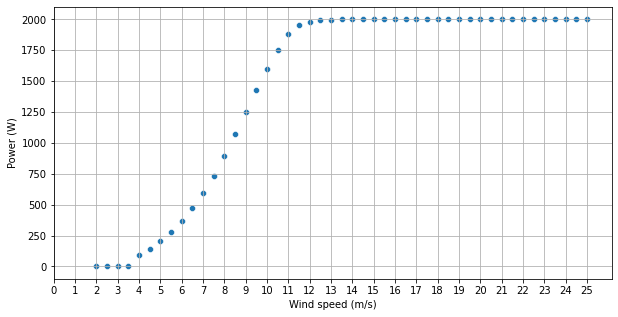
\includegraphics[scale=0.6]{Appendix1/Power_curve.png}
    \end{center}
    \caption{Power curve of the Vestas turbines at an air density of 1.225 kg/m\textsuperscript{3}}
  \end{figure}